\documentclass[a4paper]{article}

\usepackage[utf8]{inputenc}
\usepackage[english]{babel}

\usepackage[font={small,it}]{caption}

\usepackage{geometry}
\geometry{
 a4paper,
 total={160mm,247mm},
 left=25mm,
 top=25mm
 }

\usepackage{amsmath}
\usepackage{amssymb}
\usepackage{mathtools}
\usepackage{nicefrac}

\usepackage{graphicx}
\graphicspath{{./imgs/}}

\usepackage{hyperref}
\hypersetup{
	colorlinks=true,      
	urlcolor=blue,
	linkcolor=black,
	citecolor=black,
}

\setlength\parindent{0pt} % Removes all indentation from paragraphs

\title{\vspace{-15mm} The \texttt{lammps\_multistate\_rods} library \\
\vspace{5pt} \large User Manual
\vspace{20pt}
}

\author{
\text{Eugen Ro{ž}i{ć}}
}

\date{\today}

\begin{document}

\maketitle

\section{Introduction}

This library enables running hybrid MD-MC simulations in LAMMPS of interacting rods that can assume
multiple states. The dynamics of the system, as a fast process, is the MD part of the simulation, thus
enabling the full potential of LAMMPS to be used, while the changes in the (internal) states of the rods,
as a slow process, can be implemented as batches of $N$ MC moves every $M$ MD steps (this makes the most
sense in general, but the user can vary this arbitrarily).
Each MC move is consisted of choosing a rod and a new allowed state for that rod at random and then
accepting the new state of the system with probability
\begin{equation}
	P_{i \rightarrow j} = \max\left\{e^{-\left(\Delta U + \Delta \mu_{ij}\right)},\; 1\right\},
\end{equation}
where $\Delta U$ is the change in the interaction potential energy of the system and $\Delta \mu_{ij}$ is
an energy penalty due to the change in the internal state of the rod.

\vspace{1em}

The library provides a way to define a rod model which is then used to create the rods for the
simulation. Each rod is consisted of a certain number of beads (particles) and \textbf{a state of a
rod} is defined by the types of those beads, so a change in the state of a rod results in the change of
the types of the beads (particles) a rod is consisted of. Since interactions in LAMMPS are defined
through particle (bead) types this change of a rod's state results in a change in the interaction
potential energy of the system and different dynamics.

\subsection{Defining a model}

A rod model is given by a textual configuration file and it defines the geometry and mass of the rods,
all possible states a rod can assume, the interactions between rods and the transition penalties between
different rod states.\footnote{All other interactions, e.g. between rod beads and other non-rod particles
in the system, have to be given explicitly to LAMMPS in the program/input script.}

\vspace{1em}

The configuration file has the syntax of a Python file that is restricted to one-line commands, with an
exception of lines ending with a comma. The file is interpreted one line at a time in a protected environment
in the process of creation of a \texttt{Rod\_params} instance.
Some variables have special meaning as parameters of the model and their values will be kept in the
\texttt{Rod\_model} instance, others can be defined for auxiliary purposes in the configuration file itself
and will be discarded after a \texttt{Rod\_model} instance has been created.

An example of a configuration file with all possible parameters explicitly set can be found in the
\texttt{examples} directory in the library's GitHub repository
(\href{https://github.com/Saric-Group/lammps_multistate_rods}{https://github.com/Saric-Group/lammps\_multistate\_rods}).

\vspace{1em}

Through the library each rod is implemented as a small, rigid molecule that has a body, consisted of body
beads, and zero or more \textbf{patches}. A ``patch'' is a number of \textbf{interaction sites}
(particles) in a line parallel to the rod axis that share some properties. There are no intra-rod
interactions, i.e. interactions between particles/beads/interaction sites of the same rod are set to 0.
All of the geometrical parameters at the user's disposal are depicted and described in figures
\ref{img:rod_front} and \ref{img:rod_side}.

\begin{figure}[!h]
\centering
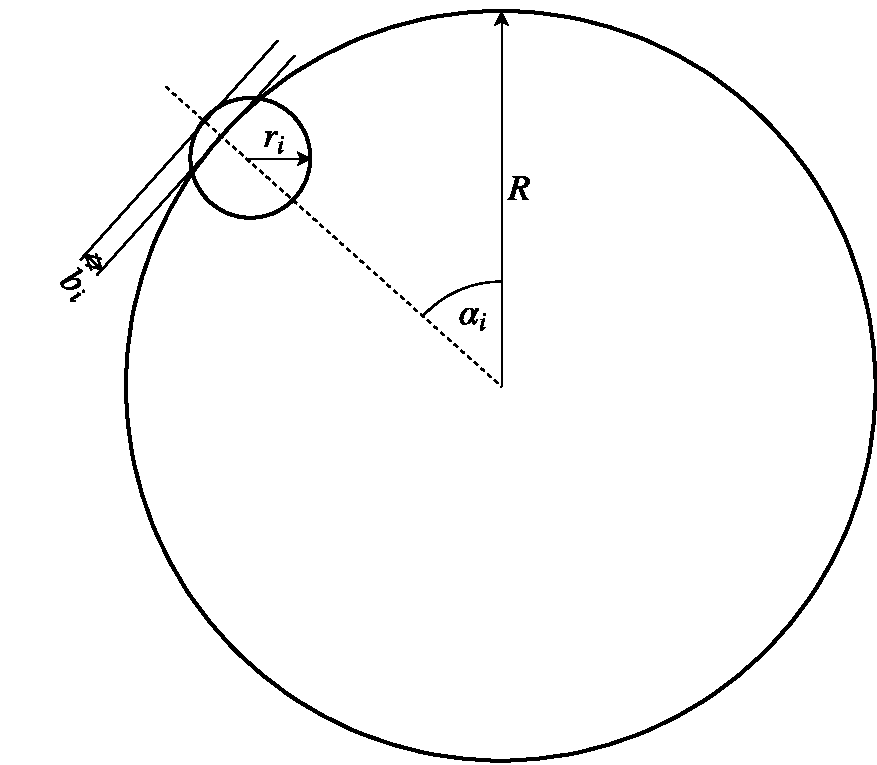
\includegraphics[width=0.38\linewidth]{rod_model-front_view.pdf}
\captionsetup{width=.7\linewidth}
\caption{A front-to-back view of an example of a rod model with one patch. In a configuration file, $R$
corresponds to the \texttt{rod\_radius} parameter and $\alpha_i$, $r_i$ and $b_i$ correspond to the
$i^\text{th}$ elements of the \texttt{patch\_angles}, \texttt{patch\_bead\_radii} and
\texttt{patch\_bulge\_out} tuples.}
\label{img:rod_front}
\end{figure}

\begin{figure}[!h]
\centering
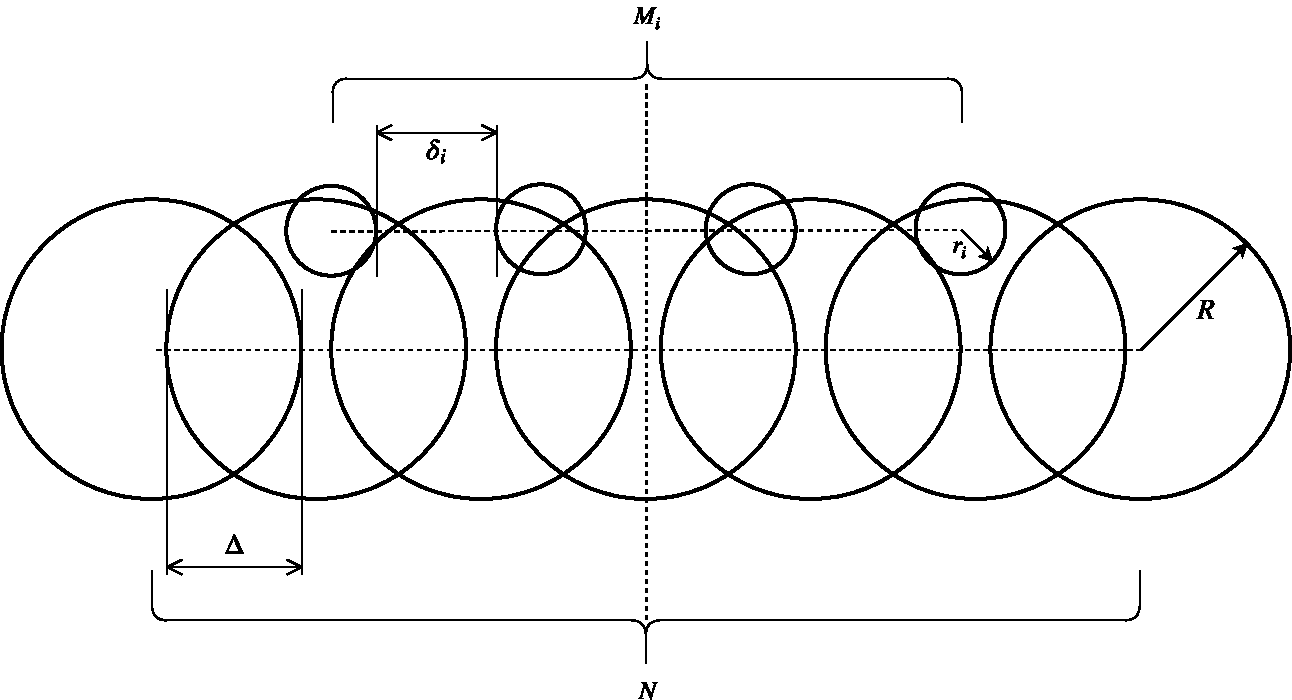
\includegraphics[width=0.7\linewidth]{rod_model-side_view.pdf}
\captionsetup{width=.7\linewidth}
\caption{A side view of an example of a rod model with one patch. In the library, $\Delta$ (the overlap
between body beads) is calculated from the \texttt{rod\_length} (from tip to tip) and
\texttt{rod\_radius} ($R$) parameters and the number of body beads $N$, which is implicitly given with
the \texttt{state\_structures} parameter; $\delta_i$ (the distance between interaction sites
in a patch) corresponds to the $i^\text{th}$ element of the \texttt{patch\_bead\_sep} tuple in the
configuration file.}
\label{img:rod_side}
\end{figure}

\vspace{1em}

Some of the features and restrictions of the model are:
\begin{itemize}
	\item The number of body beads, patches and beads in each of the patches are also set in the
	configuration file, although implicitly through the \texttt{state\_structures} parameter that also
	defines the types of all the beads in each of the states;
	\item All states have to have the same geometry (numbers and positions of beads), but some of them can
	be made \emph{inactive} (e.g. 0 interaction strength, or just volume exclusion) in some states;
	\item The parameters of an interaction are its \textbf{type} (i.e. potential function),
	\textbf{strength} and \textbf{range}, and are given separately for each pair of bead types. The
	\textbf{range} of an interaction is taken to be the distance between the \emph{surfaces} of two beads at
	which the interaction vanishes, where the \emph{surface} of a bead is taken to be the radius distance
	from its center/location.
\end{itemize}

\subsection{Running a simulation}

This library is written in Python 2.7 and uses the Python wrapper of the LAMMPS library interface
(\texttt{PyLammps}) to communicate with the LAMMPS program. In order to use it the user first has to make
a Python script that imports the \texttt{lammps} module and create an instance of \texttt{PyLammps} which
they will afterwards use in essentially the same way as in a standard textual input script.

Secondly, the user has to construct a \texttt{Rod\_model} object using a \texttt{Rod\_params}
instance which was previously instantiated and used to parse the model configuration file.
This \texttt{Rod\_model} object holds all data from the configuration file and a lot of additional,
inferred ones that instances of the \texttt{Simulation} class use, but can also come in handy to the
user. These two objects (a \texttt{PyLammps} and a \texttt{Rod\_model} instance) can then be used to
instantiate a \texttt{Simulation} object.

\vspace{1em}

The idea of the library is for it to be used to create and manipulate the (states of the) rods as
independently as possible of any other particles or features in LAMMPS. To this end the
\texttt{Simulation} class offers various convenience methods for setting up and querying the LAMMPS
simulation, creating the rods and (un)setting fixes that define the behavior of the rods.

All other elements and features of the simulation (not related to the rod objects) can be created and
set independently of the library using the \texttt{PyLammps} object, as one would normally do in a
LAMMPS (Python) input script.

\vspace{1em}

After a \texttt{Simulation} object is created and some basic properties of the simulation (e.g. units,
dimensions, boundaries etc.) set, the \texttt{setup} method should be called with some information about
all the other non-rod LAMMPS elements (particles, interactions, etc.) that are or will be used in the
simulation. This way the library takes care of everything else for the user and it is ensured no
conflicts between the rod and non-rod aspects of the simulation arise.

Next the rods can be created in various (documented) ways with the \texttt{create\_rods} method, but also
the \emph{gcmc} fix of the \texttt{set\_state\_concentration} can be used for such a purpose too.

The library offers methods to set up 3 main types of behaviors of rods through LAMMPS fixes, and those
are:
\begin{enumerate}
	\item \texttt{set\_rod\_dynamics} - sets the dynamics of ALL the rods through a \emph{rigid/small} fix
	of a given ensemble (if the user wants different dynamics for different groups of rods they will have to
	do it ``by hand'', but the contents of this method can be a good guide);
	
	\item \texttt{set\_state\_transitions} - sets up the change-of-state MC moves through a
	\emph{change/state} fix\footnote{This is a fix developed by me and can be found in my personal fork of
	LAMMPS, it is not yet available in the official LAMMPS, but it probably will be in the near future}
	using the information from the rod model (allowed transitions and corresponding penalties) 
	
	\item \texttt{set\_state\_concentration} - sets up a \emph{gcmc} fix (only for insert/delete moves) to
	keep (approximately) constant concentration of rods of a given state in the simulation (currently
	available only for one state because of the limitations of the \emph{rigid} fixes)
\end{enumerate}

The user can also define additional behaviors relating to the rod objects outside of using
the methods of the library / \texttt{Simulation} object, but should be very careful with that and
familiarise themselves beforehand with the inner workings of the (relatively well documented) library
classes.

\vspace{1em}

A demonstration of all of this and an example of how the library can be used can be found in the
\texttt{examples} directory in the form of a console application (\texttt{simulate\_nvt.py}).

\subsubsection*{Technical limitations and development points}

\begin{enumerate}
	\item Energy minimization algorithms from LAMMPS cannot be used on the rods because they are defined as
	rigid objects. However, random initial configurations can be generated in multiple other ways:
	\begin{itemize}
		\item using the \emph{random} option of the \texttt{create\_rods} method (advisably with the
		\emph{overlap} and \emph{maxtry} keywords)
		
		\item using the \emph{gcmc} fix of the \texttt{set\_state\_concentration} method in an initial
		``equilibration'' run with state-changing disabled, etc.
	\end{itemize}
\end{enumerate}

\end{document}
